\chapter{Preliminary work}
\label{sec:preliminary-work}

\section{Basic hard segmentation}
\label{sec:basic-segmentation}

The first attempt for foreground extraction was done by using segmentation algorithms \textit{Watershed} \cite{watershed} and \textit{GrabCut} \cite{grabcut} and by using basic thresholding and filtering on the Kinect depth-map.
\par
The Kinect depth-map values are thresholded based on a pre-set maximum depth in order to get a rough estimation of the foreground (Figure \ref{fig:depth-pre-f}b). Because the result though cannot be used directly due to noise in the depth-map, the thresholded depth-map was preprocessed using a blurring filter. Then a binary threshold operation was used, to convert all the foreground values to a single one in order to create a binary mask (Figure \ref{fig:depth-pre-f}c) that was further used to map the pixels in the colour image (Figure \ref{fig:results-pre-f}b).
\par
A Watershed segmentation algorithm takes the gradient of the grayscale image and considers high intensities as maxima and low intensities as minima. Maxima and minima form "valleys" and "peaks" in an image and by using a flooding technique valleys are flooded and to avoid valleys from being connected, "walls" are built on the boundaries and at the end of the process those walls produce the segmented image. Image that has many valleys/peaks and noise would produce many such walls, resulting in a bad segmentation, so usually markers are introduced to define which valleys to be merged for a better segmentation results (Figure \ref{fig:water-f}). In our case, the binary mask that was calculated in the previous method, was used as a marker parameter in the OpenCV function watershed. To create the marker parameter, the binary mask was \textit{eroded} and \textit{dilated} and then the results of these operations were combined in order to mark the boundaries of the foreground region that would be segmented by the watershed algorithm (Figure \ref{fig:depth-pre-f}d). Erosion and dilation are morphological operators that process images based on shapes within them. A kernel is used in order to remove or add boundary pixels around a shape in an image (Figure \ref{fig:dilation-f}). The kernel is usually a 3x3 cross but others can be used, and the centre pixel serves as an anchor point on the shape boundary such that the rest of the pixels in the kernel denote whether pixels should be added or removed depending on the operation. The magnitude of the operations is set based on the iterations the process runs.

\begin{figure}[t]
\centering
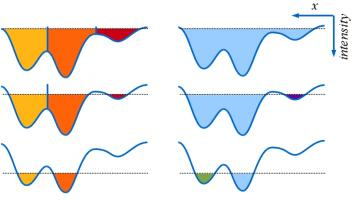
\includegraphics[width=0.7\columnwidth]{Chapter4/4/watershed.jpg}
\caption[Watershed flooding algorithm illustration.]{\textit{Watershed} flooding algorithm illustration. Valleys are flooded and "walls" are built in order to separate the regions (left). The user can specify valleys that are considered similar or noise to be connected during the flooding process (right).}
\label{fig:water-f}
\end{figure}

\begin{figure}[t]
\centering
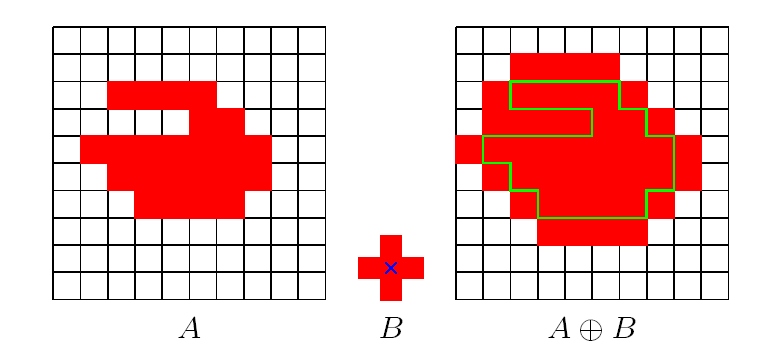
\includegraphics[width=0.8\columnwidth]{Chapter4/4/dilation.png}
\caption[Dilation on a binary image.]{\textit{Dilation} is a moprhological operator that uses a kernel to add pixels on a shape boundaries. The blue cross denotes the anchor point with the shape boundary and the rest of the pixels in the kernel denote pixels to be added.}
\label{fig:dilation-f}
\end{figure}

\par
Grabcut is a segmentation tool developed by Microsoft Research in 2004. The user specifies a bounding box around the object to be segmented (Figure \ref{fig:grab-f}) and and the colour distributions of the object and the background are modelled as Gaussian Mixture models based on the fact that everything outside the box is definite background. A graph is build based on the distributions where foreground and background nodes are connected to their corresponding foreground and background super-nodes and by using an energy minimization approach and iterated graph cuts, the foreground is hard segmented (Figure \ref{fig:graph-f}). The method has further optimizations where a user can denote with scribbles erroneously classified regions (Figure \ref{fig:grab-f}) and the process re-runs with this additional information. GrabCut has also a border matting component that softens the segmented object's boundary. In order to automate the process we took the binary mask generated from the depth-map, found the largest contour in the image using OpenCV findContour, then based on that contour we found the minimum and maximum coordinates from left to right and top to bottom and used them to create a bounding box around the foreground (Figure \ref{fig:depth-pre-f}d). Then we passed it to OpenCV's grabcut function along with the colour image to get the segmentation result.

\begin{figure}[t]
\centering
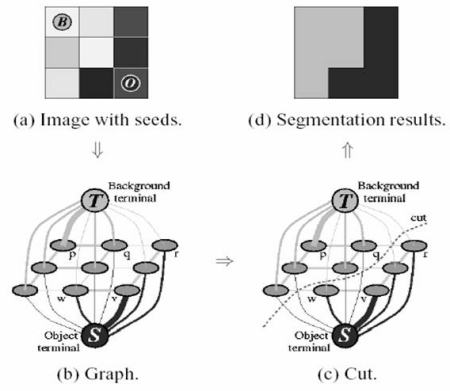
\includegraphics[width=0.6\columnwidth]{Chapter4/4/graphcut.jpg}
\caption[Graph cuts segmentation.]{\textit{GrabCut} uses graph cuts in-order to segment the image. Figure taken from \cite{grabcut}.}
\label{fig:graph-f}
\end{figure}

\begin{figure}[t]
\centering
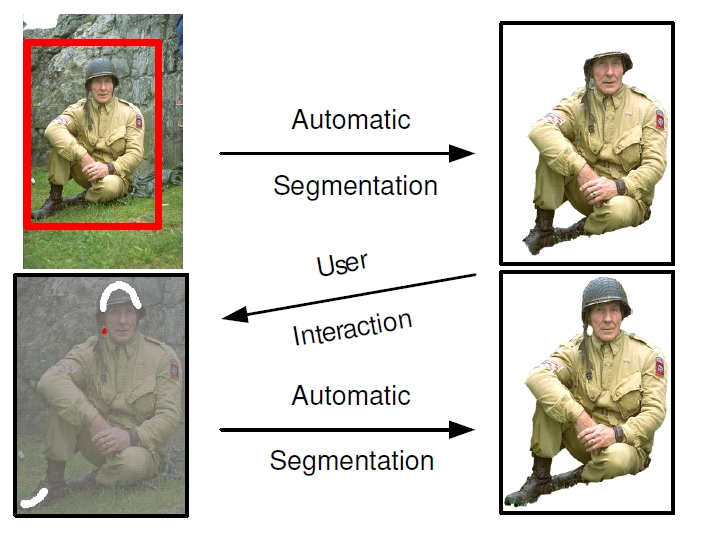
\includegraphics[width=0.6\columnwidth]{Chapter4/4/grabcut.png}
\caption[GrabCut example.]{\textit{GrabCut} has a simple interface for foreground extraction but usually need additional user input to get a good result. The user specifies a bounding box around the object to be segmented and then provides scribbles on erroneous regions as additional input. Figure taken from \cite{grabcut}.}
\label{fig:grab-f}
\end{figure}

\par
The results in general were not acceptable, even in images with a simple background (Figure \ref{fig:results-pre-f}). This was primary due to the fact that the depth-map contained too many errors, the watershed algorithm could not segment the image correctly based on the markers provided, and the grabcut algorithm needed additional user input in order to fix the erroneous regions.

\begin{figure}[t]
\centering
\subfloat[][Thresholded depth]{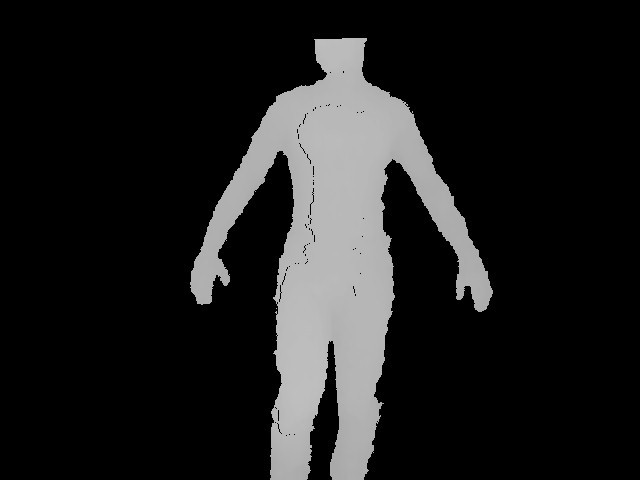
\includegraphics[width=0.4\columnwidth]{Chapter4/4/depth.jpg}}
\subfloat[][Binary mask]{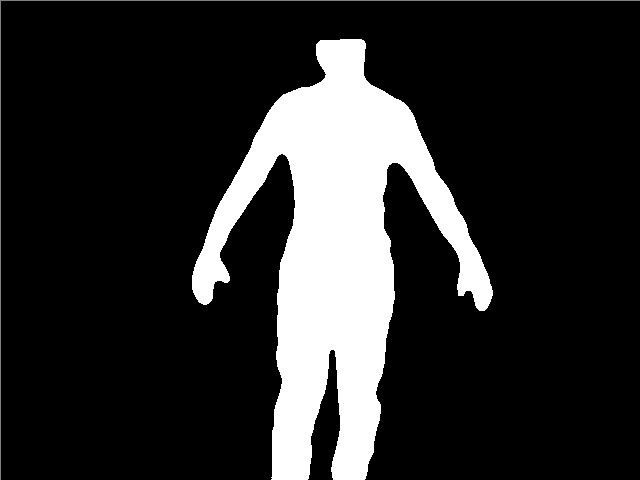
\includegraphics[width=0.4\columnwidth]{Chapter4/4/binary.jpg}}
\newline
\centering
\subfloat[][Markers]{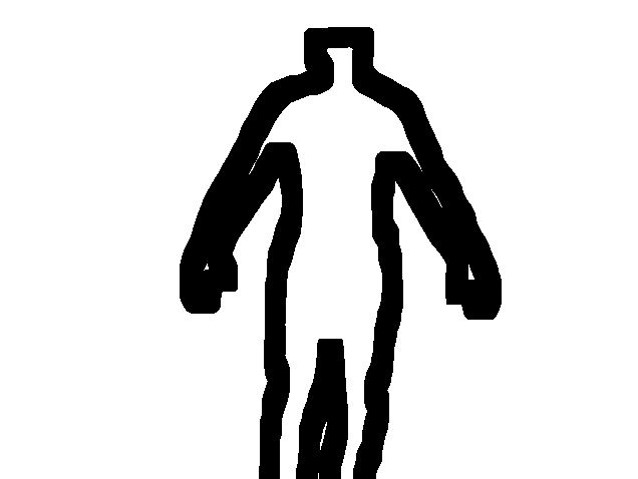
\includegraphics[width=0.4\columnwidth]{Chapter4/4/markers.jpg}}
\subfloat[][Bounding box]{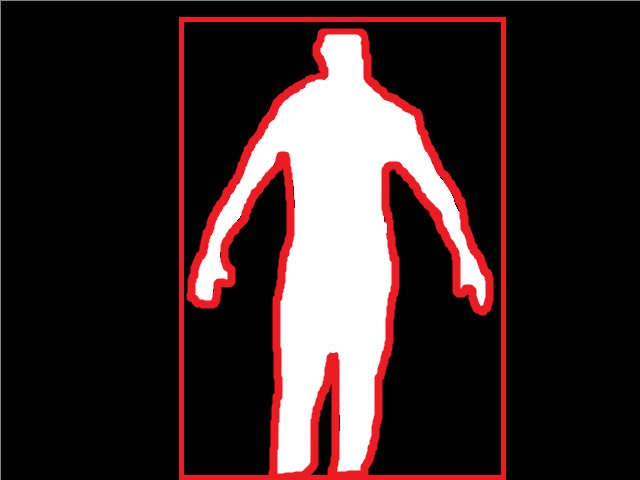
\includegraphics[width=0.4\columnwidth]{Chapter4/4/depth_box.jpg}}
\caption[Depth-map pre-processing for various methods.]{Depth-map pre-processing for various methods. A binary mask is generated from the thresholded depth to be used for compositing. The binary mask is further used to create markers for the Watershed method and to create a bounding box for the GrabCut method.}
\label{fig:depth-pre-f}
\end{figure}

\begin{figure}[t]
\centering
\subfloat[][RGB image]{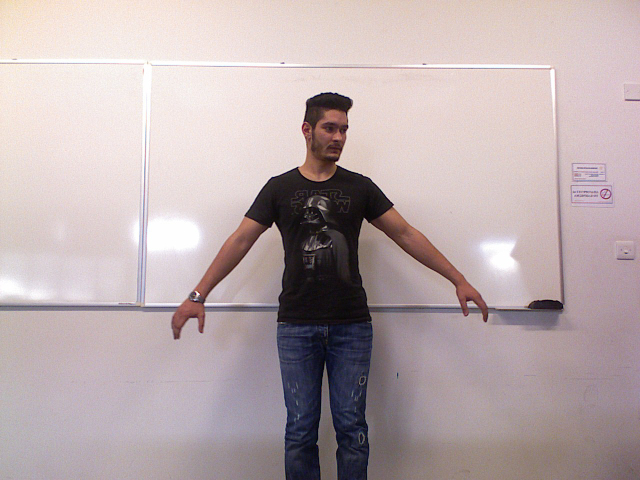
\includegraphics[width=0.4\columnwidth]{Chapter4/4/image1.jpg}}
\subfloat[][Depth-map bluring result]{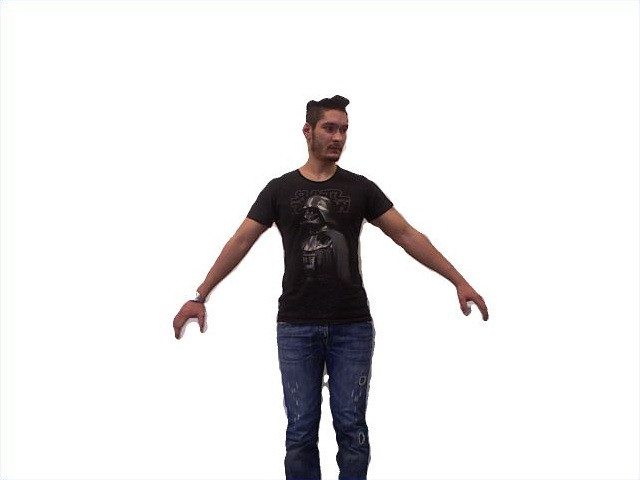
\includegraphics[width=0.4\columnwidth]{Chapter4/4/blur1.jpg}}
\newline
\centering
\subfloat[][Watershed result]{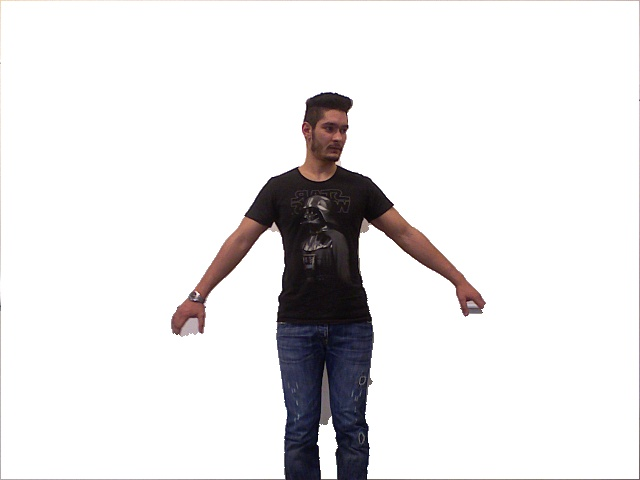
\includegraphics[width=0.4\columnwidth]{Chapter4/4/water1.jpg}}
\subfloat[][GrabCut result]{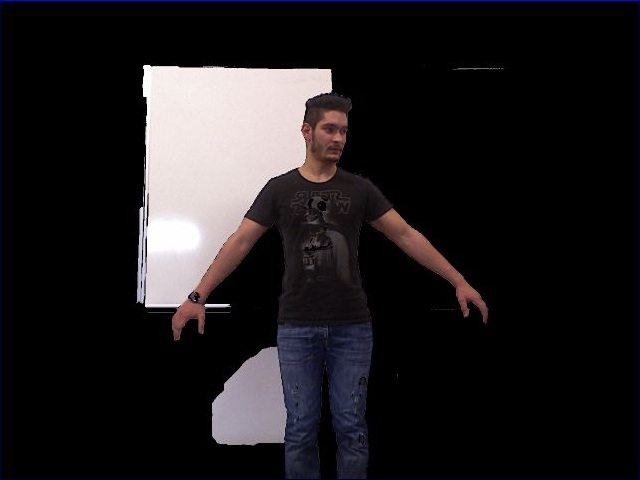
\includegraphics[width=0.4\columnwidth]{Chapter4/4/grab1.jpg}}
\caption[Results from various segmentation methods.]{Results from crating a binary mask from the depth-map (b) and from segmentation methods Watershed (c) and GrabCut (d).}
\label{fig:results-pre-f}
\end{figure}

%%%%%%%%%%%%%%%%%%%%%%%%%%%%%%%%%%%%%%%%%%%%%%%%%%%%%%%%%%5
\section{Machine learning segmentation}
\label{sec:learning-segmentation}

The next attempt was a manual approach to segmentation, were machine learning algorithms \textit{K-Nearest Neighbours} and \textit{Support Vector Machines} were used to classify pixels into foreground and background.
By providing a machine learning algorithm with foreground and background samples and their corresponding classes, pixels could be classified into foreground or background class and the result would eventually be a binary mask.
\par
The K-Nearest Neighbour algorithm is a supervised learning algorithm. Assume that we have a set of multiple items. Each item is labelled and belongs to a certain class. When a new item is added to the set it is labelled according to its similarity with the other items. This similarity is measured by its distance from the other items in a feature space. For example, in Figure \ref{fig:knn-space-f} the new item (in green) is classified based on its distance from the other items. The value of K is crucial for classification, since as illustrated in the Figure \ref{fig:knn-space-f}, two different values of K produce different classification results. The number K should always be odd in order to avoid ties.

\begin{figure}[t]
\centering
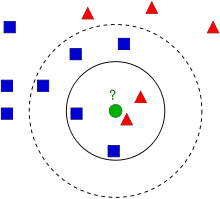
\includegraphics[width=0.5\columnwidth]{Chapter4/4/knn.png}
\caption[KNN 2-D sample space visualization.]{In \textit{K-Nearest Neighbours}, when a new item is added to the set, it is classified based on the K nearest samples to it.}
\label{fig:knn-space-f}
\end{figure}

Support vector machines is also a non-probabilistic supervised learning algorithm. Assuming again that we have a set of items, they are separated into classes using a hyperplane. The optimal hyperplane is the one that separates the items by having a maximum margin from all of them (Figure \ref{fig:svm-space-f}). Since data cannot always be separated linearly, an extension to the algorithm re-classifies misclassified items by considering the distance of items from the outer margin of the hyperplane.

\begin{figure}[t]
\centering
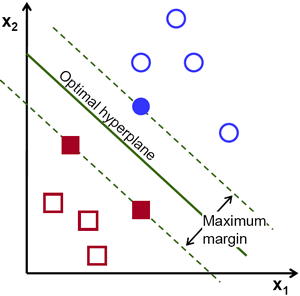
\includegraphics[width=0.5\columnwidth]{Chapter4/4/svm.png}
\caption[SVM 2-D sample space visualization.]{In \textit{Support Vector Machines}, a line that is considered the hyperplane in 2D space, optimally separates the data by considering the largest possible margin between sample sets.}
\label{fig:svm-space-f}
\end{figure}

In order to be able to provide training samples to the machine learning algorithms, we needed to create a trimap that would contain definite foreground, definite background and unknown regions. This was done by using the binary mask that had been produced in previous methods. The binary mask was eroded and dilated and the resulting masks were combined in-order to create a trimap. The basic sampling strategy was to take all the foreground and all the background pixels as training sets, but this would contribute to high running times. To solve this problem we created a new trimap that had two extra regions that were created by eroding and dilating the binary mask with a higher magnitude this time and by adding the previous masks with the two new ones to create a five-region map. Initially, all the pixels in the two extra regions were sampled to be used for training purposes and RGB values were used as features. 
\par
OpenCV includes a machine learning module that has implementations of KNN and SVM, and were used for the classification process. We provided them with the training sample sets and their corresponding classes in order to train the algorithms, and then iterated for each unknown pixel to classify it. The results weren't satisfactory and running times were still high, so by assuming that pixels close to each other have similar attributes, we used a local sampling approach by sampling pixels within a circle around the unknown pixel (Figure \ref{fig:old-method-f}). By sampling N random samples within the circle instead of all, we managed to reduce running times even more.
Tests were run with global and local sampling, on images with various foregrounds and backgrounds and the best approach was local sampling with KNN (Figure \ref{fig:results-machine-f}b). SVM failed to classify many of the unknown pixels even with an easy background (Figure \ref{fig:results-machine-f}a). KNN failed to correctly classify pixels in images with a difficult background (Figure \ref{fig:results-machine-f}d).

\begin{algorithm}
\caption{Sampling K random samples within a circle.}\label{old-sampling-method}
\begin{algorithmic}[1]
\ForAll{unknown pixels}
\ForAll{foreground and background pixels in circle}
\State F sample set $\gets$ get N random foreground samples
\State B sample set $\gets$ get N random foreground samples
\EndFor
\EndFor
\State Classification
\end{algorithmic}
\end{algorithm}

\begin{figure}[t!]
\centering
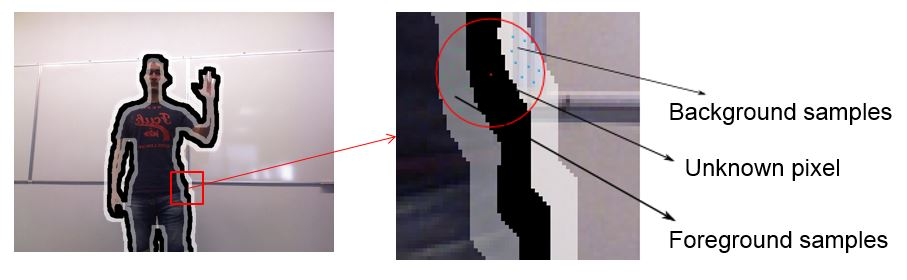
\includegraphics[width=1\columnwidth]{Chapter4/4/old_method.jpg}
\caption[Old sampling strategy.]{Five region map and sampling scheme. The five region map was an extension of the trimap that has two additional regions used for sampling. The sampling was done by selecting random samples within a radius around the unknown pixel.}
\label{fig:old-method-f}
\end{figure}

\begin{figure}[t]
%\centering
\subfloat[][SVM result]{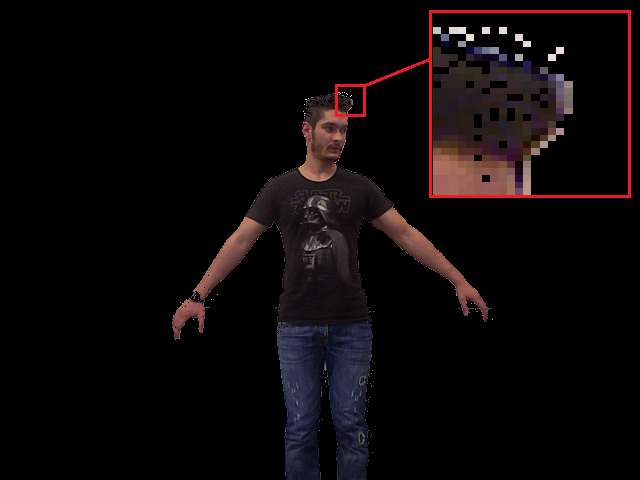
\includegraphics[width=0.5\columnwidth]{Chapter4/4/local_nonlinear_svm__result2.png}}
\subfloat[][KNN result]{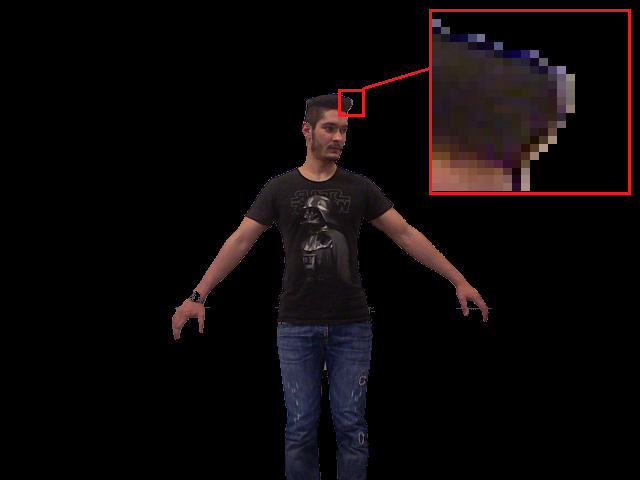
\includegraphics[width=0.5\columnwidth]{Chapter4/4/local_random_knn.png}}
\newline
\subfloat[][RGB image]{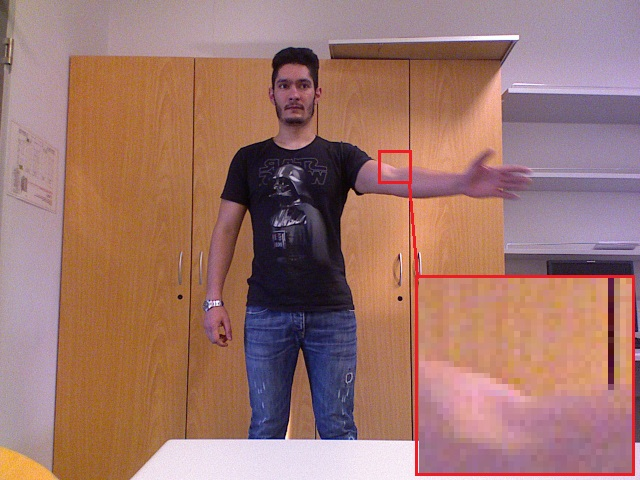
\includegraphics[width=0.5\columnwidth]{Chapter4/4/image2.png}}
\subfloat[][KNN result]{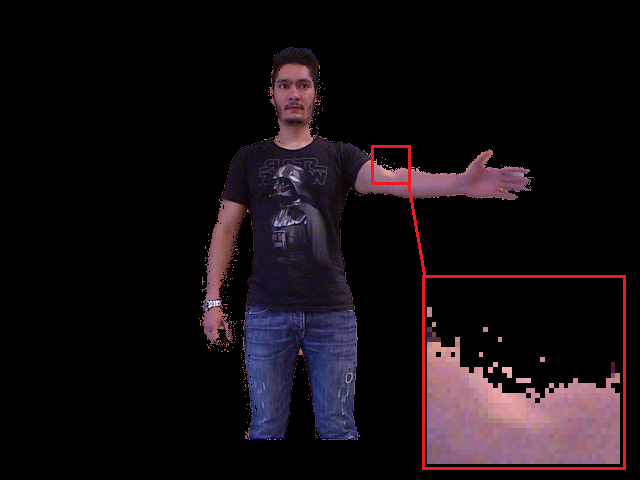
\includegraphics[width=0.5\columnwidth]{Chapter4/4/local2_random_knn.png}}
\caption[Results from machine learning based segmentation.]{For both methods sampling is local and KNN produces a better segmentation result than SVM. For a difficult background though, the KNN fails to classify many pixels resulting in a noisy boundary.}
\label{fig:results-machine-f}
\end{figure}

%%%%%%%%%%%%%%%%%%%%%%%%%%%%%%%%%%%%%%%%%%%%%%%%%%%%%%%%%%%%%%%%
\section{Early alpha matting}
\label{sec:early-matting}

At this point we considered using the matting equation that could produce the fuzzy alpha values that give a better representation of the mixed pixels in the image. In images taken from the Kinect, these kind of pixels were usually found in the boundaries of the foreground.
The matting equation requires a foreground value, a background value and the unknown pixel value in order to produce the $\alpha$ value. Since our previous approach classified a pixel into a certain class and didn't return the values of the best matching foreground and background pixels, we devised a pixel differencing method that returned the best foreground and background values that were needed to produce the $\alpha$ values.
Similarly to KNN, we formed a feature vector for each pixel that consisted of colour and spatial information, and each of the foreground and background samples feature vectors were differenced with each unknown pixel feature vector. From each of the foreground and background distance sets the K smallest differences where selected and were thereafter averaged to get the final values that would be used in the matting equation for $\alpha$ estimation.

\begin{algorithm}
\caption{Pixel differencing and averaging of best foreground and background samples.}\label{differencing-method}
\begin{algorithmic}[1]
\State Sampling
\ForAll{unknown pixels}
\ForAll{foreground samples}
\State distances set $\gets$ Difference(F, U)
\Comment{Absolute value of difference}
\EndFor
\State K smallest set $\gets$ GetSmallest(distances set)
\State F $\gets$ Average(K smallest set)
\ForAll{background samples}
\State distance set $\gets$ Difference(B, U)
\Comment{Absolute value of difference}
\EndFor
\State K smallest set $\gets$ GetSmallest(distances set)
\State B $\gets$ Average(K smallest set)
\EndFor
\end{algorithmic}
\end{algorithm}

For problematic regions with overlapping colour distributions we used \textit{Local Binary Patterns} \cite{lbp} as an extra feature. Local binary patterns are binary codes that represent a pixels texture. Figure \ref{fig:lbp-m-f} illustrates the process for computing the LBPs. The results weren’t improved mainly due to the fact that LBP provide general information about an image texture, usually via a histogram, and not pixel based information, LBPs failed to separate regions with similar colours but different texture (Figure \ref{fig:lbp-f}).

\begin{figure}[t]
\centering
\includegraphics[width=0.8\columnwidth]{Chapter4/4/lbp.jpg}
\caption[Local binary patterns computation methodology.]{\textit{Local binary patterns} are computed on the grayscale image.}
\label{fig:lbp-m-f}
\end{figure}

\begin{figure}[t]
\centering
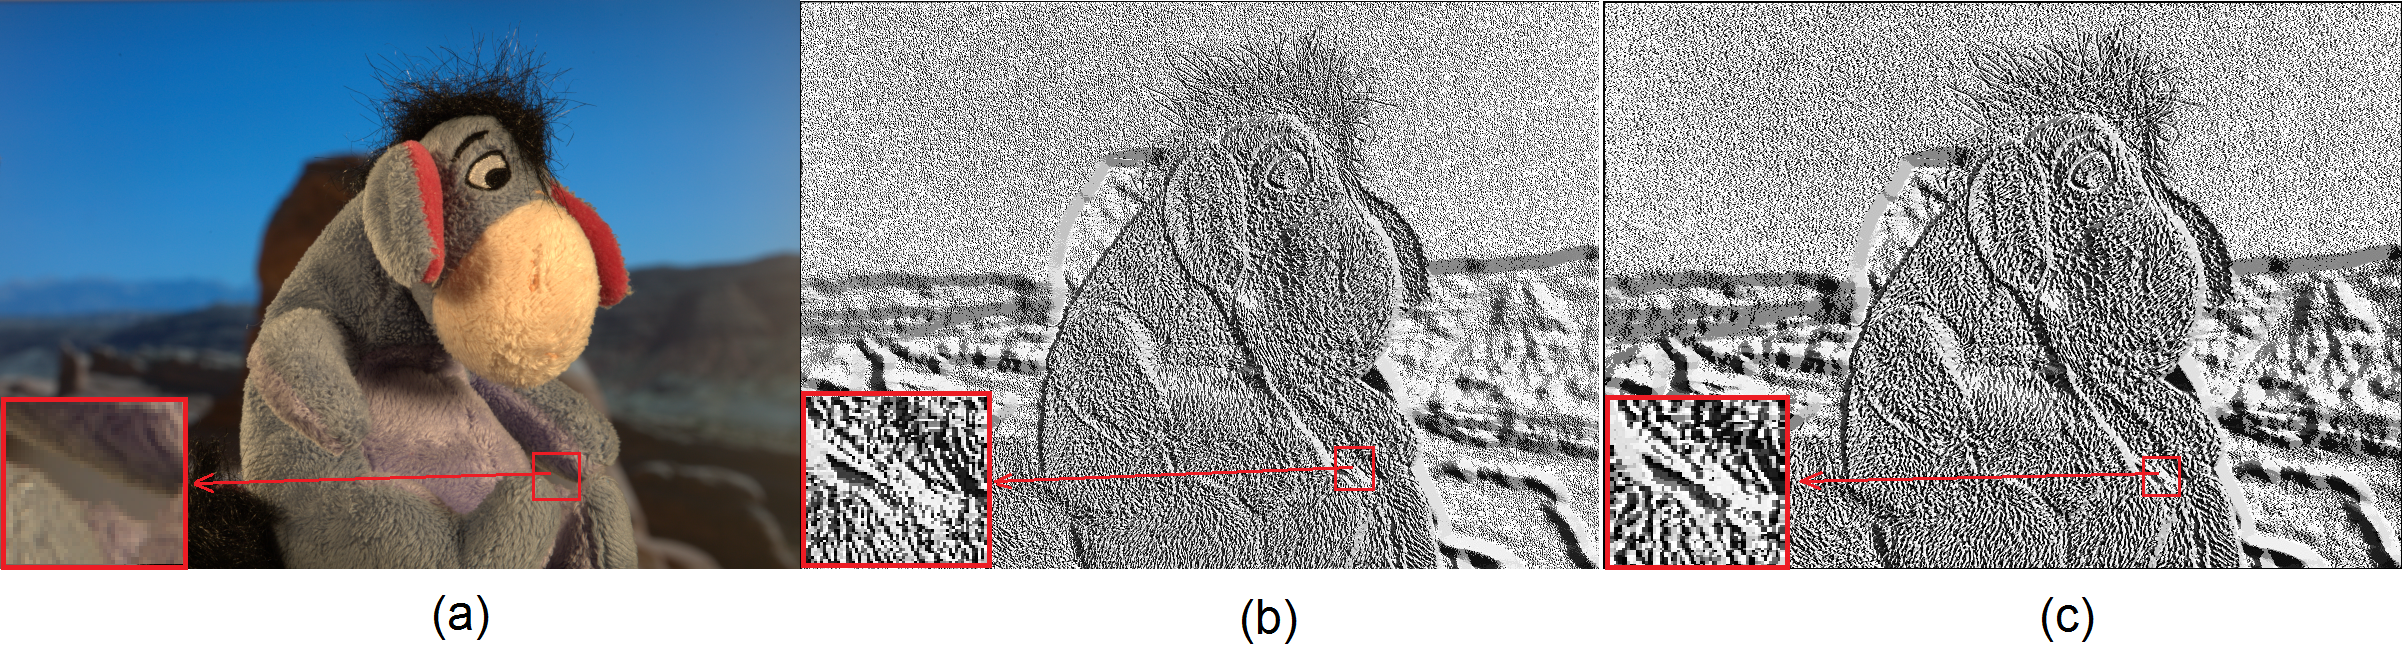
\includegraphics[width=1\columnwidth]{Chapter4/4/lbp_figure.jpg}
\caption[Local binary patterns visualization.]{Local binary patterns images, produced by an 8x8 window (b) and 16x16 window (c). LBP fails to separate regions with similar colours but different texture in the image version of them.}
\label{fig:lbp-f}
\end{figure}

Since LBP did not solve the problem of overlapping F and B colour distributions, we re-assessed the problem and observed that colour images taken from the Kinect, had colour distortion due to jpeg compression and this contributed to the problem of miss-classified pixels. To tackle this issue we used the \textit{Kuwahara filter} that is an noise reducing, edge preserving filter. The Kuwahara filtering algorithm uses sliding window over each pixel and uses the variance of the mean of surrounding pixel regions in order to determine the value of the centre pixel. For colour images the variance is determined from the brightness channel of the HSV colour space and the colour channel values are determined by the mean the pixels in the region with the least variance for each colour channel.
This preprocessing work helped reduce miss-classified pixels that were far from from their corresponding region but it produced some artifacts on the edges of the foreground that caused misclassification of other pixels. Also the Kuwahara filter is a non-linear filter that produced an overhead in running times for high resolution images.

\begin{figure}[t]
\centering
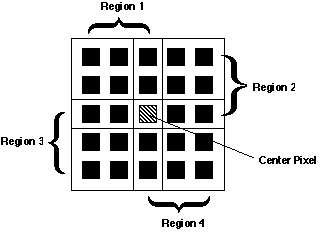
\includegraphics[width=0.6\columnwidth]{Chapter4/4/kuwa.png}
\caption[Kuwahara filter window illustration.]{The \textit{Kuwahara filter} uses a sliding window, where the centre pixel value is determined by the least variance of the mean of each pixel region.}
\label{fig:kuwahara-f}
\end{figure}

\begin{figure}[t]
\centering
\includegraphics[width=1\columnwidth]{Chapter4/4/Kuwahara_figure.jpg}
\caption[Kuwahara filter example.]{The \textit{Kuwahara filter} has noise reduction and edge preserving properties.}
\label{fig:kuwahara-f}
\end{figure}

For smoothness, we used a feature that was derived from a mask that weighted unknown region values based on their distance from the foreground. The mask was created by applying a blurring filter to the binary mask (Figure \ref{fig:blur-weight-f}). The values were normalized before use and their magnitude was downgraded so they would not dominate in the feature space. The kernel size for the blurring filter was chosen to produce a blurred region that would be as wide as the unknown region. This approach worked well in cases were the total unknown region had a smooth width around the foreground region.

\begin{figure}[t]
\centering
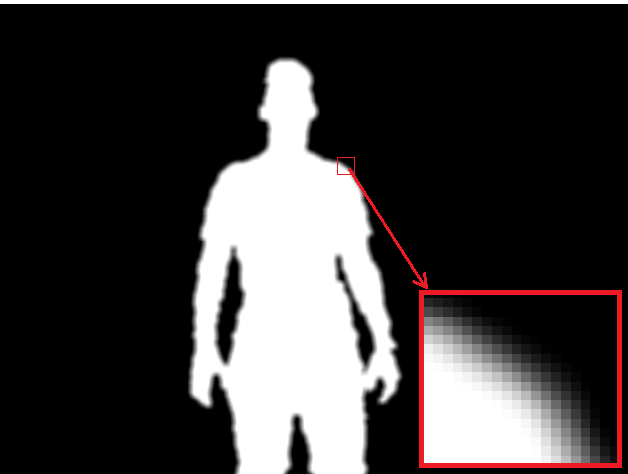
\includegraphics[width=0.8\columnwidth]{Chapter4/4/blur_weight.png}
\caption[Mask that weights the unknown pixels based on their distance from the foreground.]{Mask that weights the unknown pixels based on their distance from the foreground.}
\label{fig:blur-weight-f}
\end{figure}